\section{Specification of temporal properties}
% add section introduction here
\hspace{1cm} This section introduces approaches for specifying temporal properties 
in UML/OCL models, focusing on extensions that address OCL's limitations with temporal 
and event-based constraints. We examine Temporal OCL (TOCL) as a foundational extension, 
then introduce our TOCL+ language that enhances temporal specification with event 
constructs and bounded existence operators. The formal definitions and grammar 
provided establish a precise foundation for both specification and subsequent 
verification of temporal properties.

%%%%% TOCL
\subsection{Temporal OCL (TOCL)}

\hspace{1cm} Temporal OCL (TOCL), introduced by Ziemann and Gogolla \cite{TOCL}, 
extends the Object Constraint Language (OCL) to address a fundamental limitation: 
the inability to specify constraints that span multiple system states over time. 
While standard OCL excels at defining invariants within a single state or basic 
pre/post-condition constraints for operations, it lacks the expressiveness needed 
for complex temporal behaviors. TOCL overcomes this limitation by incorporating 
elements from linear temporal logic while preserving OCL's familiar syntax and type 
system, making it particularly valuable for modeling reactive systems, concurrent 
processes, and real-time applications where temporal reasoning is essential.

TOCL defines its semantic framework over an infinite sequence of system states 
$\hat{\sigma} = \langle \sigma_0, \sigma_1, \ldots \rangle$, where each temporal 
constraint is evaluated within an environment $\tau = (\hat{\sigma}, i, \beta)$. 
Here, $i$ represents the current state index in the sequence, and $\beta$ is a 
variable assignment. This framework enables reasoning about both the future and 
past evolution of system states, providing a comprehensive approach to temporal 
specification. Unlike standard OCL invariants that apply to a single state, TOCL 
invariants implicitly apply an "always" condition, meaning constraints must hold 
across the entire state sequence unless otherwise specified.

The expressive power of TOCL comes from its temporal operators, which enable precise 
specification of how properties evolve over time. These operators form the core of 
TOCL's extension to standard OCL, allowing constraints to reference past states, 
future states. By providing mechanisms to reason about both historical behavior and 
future evolution of the system, these operators significantly enhance OCL's ability 
to express dynamic properties.

TOCL organizes its temporal operators into two categories:

\paragraph{Future Operators:} 
\begin{itemize} 
    \item \textbf{next $e$:} True if $e$ holds in the next state (state $i+1$). 
    \item \textbf{always $e$:} True if $e$ holds in the current state and all subsequent states (all states $j \geq i$). 
    \item \textbf{sometime $e$:} True if $e$ holds in the current state or at least one future state (some state $j \geq i$). 
    \item \textbf{always $e_1$ until $e_2$:} True if $e_1$ remains true until $e_2$ becomes true. 
    \item \textbf{sometime $e_1$ before $e_2$:} True if $e_1$ becomes true at some point before $e_2$ does. 
\end{itemize}

\paragraph{Past Operators:} 
\begin{itemize} 
    \item \textbf{previous $e$:} True if $e$ was true in the previous state or if at the initial state ($i = 0$). 
    \item \textbf{alwaysPast $e$:} True if $e$ was true in all past states (all states $0 \leq j < i$). 
    \item \textbf{sometimePast $e$:} True if $e$ was true in at least one past state (some state $0 \leq j < i$). 
    \item \textbf{always $e_1$ since $e_2$:} True if $e_1$ has been true since the last time $e_2$ was true. 
    \item \textbf{sometime $e_1$ since $e_2$:} True if $e_1$ has been true at some point since the last time $e_2$ was true. 
\end{itemize}

In TOCL, the expressions $e$, $e_1$, and $e_2$ represent boolean OCL expressions 
that evaluate to either true or false within a specific system state. These 
expressions may encompass standard OCL constructs, such as attribute access, 
navigation through associations, or operations on collections. The temporal 
operators specify the conditions under which these expressions must hold across 
a sequence of states, thereby extending OCL's traditionally static constraints 
into a dynamic, temporal framework.

The semantics of TOCL's temporal operators are formally grounded in state sequences 
and set theory, providing a rigorous basis for their evaluation. Consider a state 
sequence beginning at an initial state $i = 0$. The operator \texttt{next $e$} holds 
true at state $i$ if $e$ is true at state $i+1$, while \texttt{always $e$} requires 
$e$ to hold for all states $j \geq i$. Conversely, \texttt{sometime $e$} is satisfied 
if $e$ holds for at least one state $j \geq i$. For past-oriented operators, 
\texttt{previous $e$} is true at state $i$ if $e$ held at state $i-1$, with special 
consideration at the initial state ($i = 0$). These definitions enable precise 
reasoning about temporal relationships, making TOCL a powerful tool for specifying 
and verifying system properties.

To demonstrate TOCL's capabilities, we apply it to the first two temporal properties 
from our Software System example \ref{fig:temporal_properties}:

\begin{lstlisting}[
    style=toclstyle, 
    caption={TOCL Specification for Safety Properties}, 
    label={lst:tocl_safety12},
    float=htb
]
context System 
/*
An application loading must precede its run.
*/
inv safety1: 
    self.runningApps->notEmpty() implies 
    self.runningApps->forAll(app | 
        sometimePast self.loadedApps->includes(app)
    )
/*
There must be an install operation between loading and running.
*/
inv safety2: 
    self.loadedApps->notEmpty() implies 
    self.loadedApps->forAll(app | 
        sometime self.installedApps->includes(app) 
        before self.runningApps->includes(app)
    )
\end{lstlisting}

TOCL can express properties spanning multiple states through state-based workarounds, as shown in Listing \ref{lst:tocl_safety12}. For Safety 1, rather than directly detecting the \texttt{load} operation call, TOCL uses \texttt{sometimePast} with state predicates to infer that loading occurred before running based on collection membership. Similarly, for Safety 2, TOCL uses the \texttt{before} operator with state predicates to infer the sequencing of operations through their effects on system state. While indirect, these specifications work because they only need to track the order of state changes, not count specific events.

However, TOCL fundamentally cannot specify Safety 3: \textit{"Each application can be loaded at most one time"}. This property requires counting operation call occurrences, which cannot be inferred from state changes alone. Since TOCL lacks constructs to identify when operations are called or to count events, it cannot express constraints that limit how many times an operation occurs. This limitation becomes a critical barrier when specifying common safety properties that restrict operation frequencies.
% \hspace{1cm} Temporal OCL (TOCL), introduced by Ziemann and Gogolla \cite{TOCL}, 
% extends the Object Constraint Language (OCL) to address a fundamental limitation: 
% the inability to specify constraints that span multiple system states over time. 
% While standard OCL excels at defining invariants within a single state or basic 
% pre/post-condition constraints for operations, it lacks the expressiveness needed 
% for complex temporal behaviors. TOCL overcomes this limitation by incorporating 
% elements from linear temporal logic while preserving OCL's familiar syntax and type 
% system, making it particularly valuable for modeling reactive systems, concurrent 
% processes, and real-time applications where temporal reasoning is essential.

% TOCL defines its semantic framework over an infinite sequence of system states 
% $\hat{\sigma} = \langle \sigma_0, \sigma_1, \ldots \rangle$, where each temporal 
% constraint is evaluated within an environment $\tau = (\hat{\sigma}, i, \beta)$. 
% Here, $i$ represents the current state index in the sequence, and $\beta$ is a 
% variable assignment. This framework enables reasoning about both the future and 
% past evolution of system states, providing a comprehensive approach to temporal 
% specification. Unlike standard OCL invariants that apply to a single state, TOCL 
% invariants implicitly apply an "always" condition, meaning constraints must hold 
% across the entire state sequence unless otherwise specified.

% A notable feature of TOCL is its treatment of operations through "process types", 
% which represent operations as entities existing only in two consecutive states: 
% before and after execution. Each operation in a class has a corresponding process 
% type that exists across these two states—the pre-state where the process instance is 
% "new" (\texttt{process.oclIsNew()} is true), and the post-state after the operation 
% completes. This mechanism allows TOCL to track operation occurrences and their 
% effects on the system state. While TOCL reuses OCL's navigation 
% expressions, collection operations, and quantifiers, it extends these with temporal 
% capabilities that span multiple states rather than being limited to a single snapshot.

% The expressive power of TOCL comes from its temporal operators, which enable precise 
% specification of how properties evolve over time. These operators form the core of 
% TOCL's extension to standard OCL, allowing constraints to reference past states, 
% future states, and temporal relationships between events. By providing mechanisms 
% to reason about both historical behavior and future evolution of the system, these 
% operators significantly enhance OCL's ability to express dynamic properties.

% TOCL organizes its temporal operators into two categories:

% \paragraph{Future Operators:} 
% \begin{itemize} 
%     \item \textbf{next $e$:} True if $e$ holds in the next state (state $i+1$). 
%     \item \textbf{always $e$:} True if $e$ holds in the current state and all subsequent states (all states $j \geq i$). 
%     \item \textbf{sometime $e$:} True if $e$ holds in the current state or at least one future state (some state $j \geq i$). 
%     \item \textbf{always $e_1$ until $e_2$:} True if $e_1$ remains true until $e_2$ becomes true. 
%     \item \textbf{sometime $e_1$ before $e_2$:} True if $e_1$ becomes true at some point before $e_2$ does. 
% \end{itemize}

% \paragraph{Past Operators:} 
% \begin{itemize} 
%     \item \textbf{previous $e$:} True if $e$ was true in the previous state or if at the initial state ($i = 0$). 
%     \item \textbf{alwaysPast $e$:} True if $e$ was true in all past states (all states $0 \leq j < i$). 
%     \item \textbf{sometimePast $e$:} True if $e$ was true in at least one past state (some state $0 \leq j < i$). 
%     \item \textbf{always $e_1$ since $e_2$:} True if $e_1$ has been true since the last time $e_2$ was true. 
%     \item \textbf{sometime $e_1$ since $e_2$:} True if $e_1$ has been true at some point since the last time $e_2$ was true. 
% \end{itemize}

% In TOCL, the expressions $e$, $e_1$, and $e_2$ represent boolean OCL expressions 
% that evaluate to either true or false within a specific system state. These 
% expressions may encompass standard OCL constructs, such as attribute access, 
% navigation through associations, or operations on collections. The temporal 
% operators specify the conditions under which these expressions must hold across 
% a sequence of states, thereby extending OCL’s traditionally static constraints 
% into a dynamic, temporal framework. This capability allows TOCL to capture the 
% evolution of system properties over time with precision and clarity.

% % Highlighting the role of invariants in TOCL
% Temporal operators play a critical role in defining invariants within TOCL, which are constraints required to hold across an entire state sequence. By default, TOCL invariants are implicitly prefixed with the \texttt{always} operator, mandating their truth in every state unless explicitly altered by other temporal operators. This flexibility allows for the specification of complex temporal properties. For instance, \texttt{always (self.state = 'active' implies sometime self.state = 'idle')} ensures that whenever the system enters an active state, it will eventually transition to an idle state. Similarly, \texttt{always self.running since self.started} stipulates that the system remains running continuously from the moment it starts, demonstrating TOCL’s capacity to express both liveness and persistence properties.

% % Formalizing the semantics of TOCL operators
% The semantics of TOCL’s temporal operators are formally grounded in state sequences and set theory, providing a rigorous basis for their evaluation. Consider a state sequence beginning at an initial state $i = 0$. The operator \texttt{next $e$} holds true at state $i$ if $e$ is true at state $i+1$, while \texttt{always $e$} requires $e$ to hold for all states $j \geq i$. Conversely, \texttt{sometime $e$} is satisfied if $e$ holds for at least one state $j \geq i$. For past-oriented operators, \texttt{previous $e$} is true at state $i$ if $e$ held at state $i-1$, with special consideration at the initial state ($i = 0$). These definitions enable precise reasoning about temporal relationships, making TOCL a powerful tool for specifying and verifying system properties.

% % Illustrating practical applications of TOCL operators
% The practical utility of TOCL’s temporal operators is evident in their ability to specify a diverse range of system properties. For safety properties, \texttt{always not self.errorState} ensures that the system never enters an erroneous condition. Liveness properties, such as \texttt{sometime self.goalState}, guarantee that a desired state is eventually achieved. Fairness constraints, like \texttt{always sometime self.resourceAllocated}, ensure that resources are allocated repeatedly over time. A concrete example from a traffic light system, \texttt{always (self.color = 'red' implies sometime self.color = 'green')}, captures the critical liveness property that a red light must eventually be followed by a green light, illustrating TOCL’s applicability to real-world dynamic systems.


% To demonstrate TOCL's capabilities, we apply it to the first two temporal properties 
% from our Software System example \ref{fig:temporal_properties}:

% \begin{lstlisting}[
%     style=toclstyle, 
%     caption={TOCL Specification for Safety Properties.}, 
%     label={lst:tocl_safety12}
% ]
% context System 
% /*
% An application loading must precede its run.
% */
% inv safety1: 
%     self.runningApps->notEmpty() implies 
%     self.runningApps->forAll(app | 
%         sometimePast self.loadedApps->includes(app)
%     )
% /*
% There must be an install operation between loading and running.
% */
% inv safety2: 
%     self.loadedApps->notEmpty() implies 
%     self.loadedApps->forAll(app | 
%         sometime self.installedApps->includes(app) 
%         before self.runningApps->includes(app)
%     )
% \end{lstlisting}

% TOCL can express properties spanning multiple states through state-based workarounds, 
% as shown in Listing \ref{lst:tocl_safety12}. For Safety 1, rather than directly 
% detecting the \texttt{load} operation call, TOCL uses \texttt{sometimePast} with 
% state predicates to infer that loading occurred before running based on collection 
% membership. Similarly, for Safety 2, TOCL uses the \texttt{before} operator with 
% state predicates to infer the sequencing of operations through their effects on 
% system state. While indirect, these specifications work because they only need to 
% track the order of state changes, not count specific events.

% However, TOCL fundamentally cannot specify Safety 3: \textit{"Each application can 
% be loaded at most one time"}. This property requires counting operation call 
% occurrences, which cannot be inferred from state changes alone. Since TOCL lacks 
% constructs to identify when operations are called or to count events, it cannot 
% express constraints that limit how many times an operation occurs. This limitation 
% becomes a critical barrier when specifying common safety properties that restrict 
% operation frequencies.


%%%%% Event
\subsection{TOCL+: An Extension of TOCL}

\hspace{1cm} To address TOCL's limitations in expressing event-based properties, 
we propose TOCL+, which extends TOCL with explicit event specification capabilities. 
Following the synchronous paradigm, TOCL+ represents operation calls as atomic 
transitions from pre-states to post-states without intermediate states. This approach 
simplifies verification while preserving essential system behaviors.

TOCL+ introduces two primary event constructs:

1. \textbf{isCalled}: Detects when an operation is invoked on an object. It takes 
the operation call with its parameters as an argument and represents the atomic 
transition from pre-state to post-state.

2. \textbf{becomesTrue}: Represents a state change event parameterized by an OCL 
boolean expression P. It identifies transitions where P changes from false to true 
between consecutive states.

\begin{figure}[H]
    \centering
    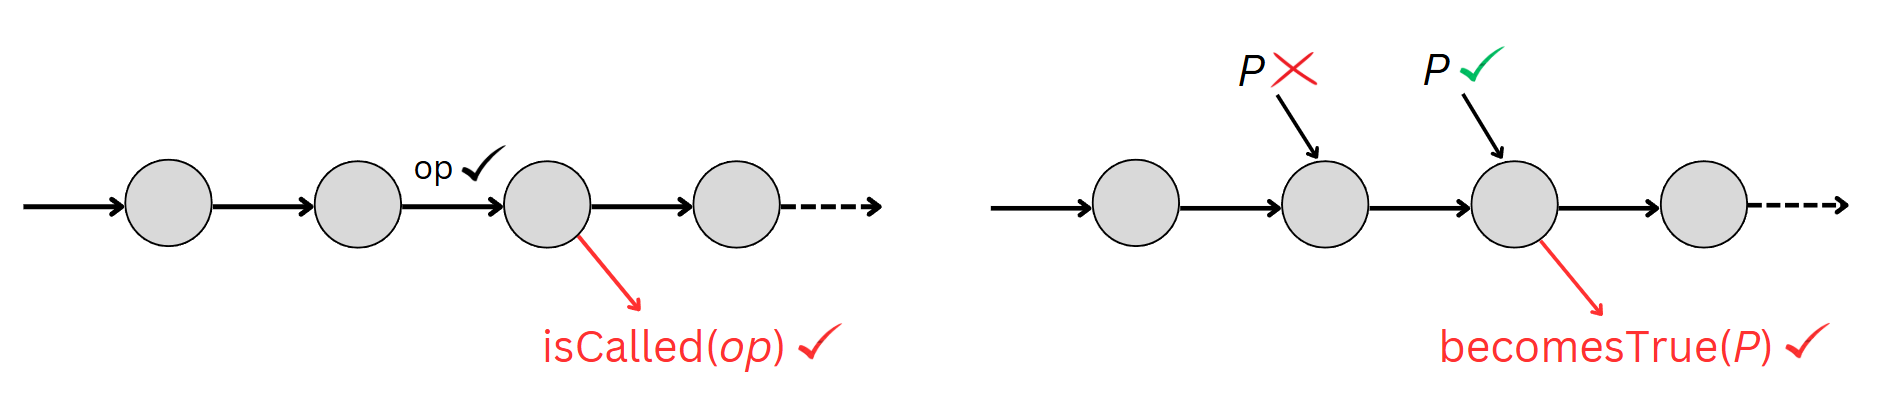
\includegraphics[width=1\textwidth]{figures/c2/events_visual.png}
    \caption{Events.}
    \label{fig:event_constructs}
\end{figure}

We adopt the concept of events from \cite{TOCL_Taha}, which defines events 
as predicates identifying specific instants in time. As discussed in Section 
\ref{sec:ocl}, object-oriented systems typically recognize operation events, 
time-triggered events, and state change events. TOCL+ focuses on operation and 
state change events as they capture the fundamental interactions in object-oriented 
systems.

In addition, TOCL+ supports bounded existence properties specifically for the 
\texttt{isCalled} event construct, allowing developers to specify constraints on 
operation call frequency:
\begin{itemize}
    \item \texttt{isCalled(...) at most \textit{k} times} - limiting operation call occurrences to no more than \textit{k}
    \item \texttt{isCalled(...) \textit{k} times} - requiring precisely \textit{k} occurrences of an operation call
    \item \texttt{isCalled(...) at least \textit{k} times} - requiring operation call occurrences to be \textit{k} or more
\end{itemize}
% In addition, TOCL+ supports bounded existence properties with constructs like:
% \begin{itemize}
%     \item \texttt{at most \textit{k} times} - limiting event occurrences to no more 
%     than \textit{k}
%     \item \texttt{exactly \textit{k} times} - requiring precisely \textit{k} 
%     occurrences of an event
%     \item \texttt{at least \textit{k} times} - requiring event occurrences to be 
%     \textit{k} or more
% \end{itemize}

Applying TOCL+ to our Software System example from Chapter 1, we can express all 
four temporal properties from Figure \ref{fig:temporal_properties}:
\begin{lstlisting}[
    style=toclstyle, 
    caption={TOCL+ Specifications}, 
    label={lst:tocl+},
    float=htb
]
context System
/*
An application loading must precede its run.
*/
inv safety1: 
    self.runningApps->notEmpty() implies
    self.runningApps->forAll(app |
        isCalled(run(app : Application)) implies
        sometimePast isCalled(load(app : Application))
    )

/*
There must be an install operation between an application's loading and its running.
*/
inv safety2: 
    self.runningApps->notEmpty() implies
    self.runningApps->forAll(app |
        isCalled(run(app : Application)) implies (
            sometime isCalled(install())
            since isCalled(load(app : Application))
        )
    )

/*
Each application can be loaded at most one time.
*/
inv safety3:
    self.installedApps->notEmpty() implies
    self.installedApps->forAll(app |
        sometimePast isCalled(load(app : Application))
        at most 1 times
    )

/*
Every loaded application will eventually be installed.
*/
inv liveness:
    self.loadedApps->notEmpty() implies
    self.loadedApps->forAll(app | 
        sometime isCalled(install())
    )
\end{lstlisting}

These examples show TOCL+'s expressive power. With the \texttt{isCalled} construct, 
safety properties 1 and 2 directly reference operation calls rather than inferring 
them from state changes. Safety property 3 uses bounded existence ("at most 1 times") 
to limit operation occurrences - something impossible in both standard OCL and TOCL. 
The liveness property also benefits from direct operation call detection, making 
the requirement clearer.


\subsection{Formal Definition for Event constructs}

\hspace{1cm} Formally, we define TOCL+ event constructs in terms of state transitions 
within the semantic framework established by TOCL. Let 
$\hat{\sigma} = \langle \sigma_0, \sigma_1, \ldots \rangle$ 
be an infinite sequence of states, and 
$\tau = (\hat{\sigma}, i, \beta)$ 
be an evaluation environment where $i$ represents the current state index and $\beta$ 
is a variable assignment.

Unlike the original TOCL approach with process types, we directly associate operation 
calls with state transitions. We assume each transition from 
$\sigma_{i-1}$ to $\sigma_i$ 
is caused by exactly one atomic operation execution, with no intermediate states.

Our event constructs are formally defined as follows:
\vspace{-1.5em}
\paragraph{isCalled(op(a$_1$, \ldots, a$_N$))}
This construct detects when an operation $op$ is invoked on an object with specific 
parameters. It evaluates to true at state $\sigma_i$ if the transition from 
$\sigma_{i-1}$ to $\sigma_i$ was caused by the operation $op$ being called on the 
context object with the specified parameters.

For an operation $op$ defined in class $C$ with parameters 
$param_1: type_1,$ $\ldots, param_N: type_N$, and context object $self$ of type $C$, 
the semantics at state $\sigma_i$ in environment $\tau = (\hat{\sigma}, i, \beta)$ 
is:
\begin{equation}
    \begin{split}
    & I[\text{isCalled}(op(a_1, \ldots, a_N))](\tau) = \text{true} \iff \\
    & \bullet\; i > 0 \text{ and} \\
    & \bullet\; \text{The transition from } \sigma_{i-1} \text{ to } \sigma_i \text{ is labeled with a call } \text{call}_i = (\omega, o, \text{args}) \\
    & \text{ where:} \\
    & \quad \circ\; \omega = \text{op} \text{ and} \\
    & \quad \circ\; o = I[\text{self}](\tau) \text{ and} \\
    & \quad \circ\; \text{args} = (I[a_1](\tau), \ldots, I[a_N](\tau))
    \end{split}
\end{equation}
% \begin{align}
%     &I[\text{isCalled}(op(a_1, \ldots, a_N))](\tau) = \text{true} \notag\\
%     &\quad \text{if and only if:}\notag\\
%     &\quad \begin{cases}
%     i > 0\\
%     \text{The transition from } \sigma_{i-1} \text{ to } \sigma_i \text{ has: }\\
%     \quad\omega = \text{op}\\
%     \quad o = I[\text{self}](\tau)\\
%     \quad\text{args} = (I[a_1](\tau), \ldots, I[a_N](\tau))
%     \end{cases}
% \end{align}

\paragraph{becomesTrue(P)}
This construct identifies transitions where a boolean expression $P$ changes from 
false to true between consecutive states.

For a boolean OCL expression $P$, the semantics at state $\sigma_i$ in environment 
$\tau = (\hat{\sigma}, i, \beta)$ is:

\begin{equation}
    \begin{split}
    & I[\text{becomesTrue}(P)](\tau) = \text{true} \iff \\
    & \bullet\; i > 0 \text{ and} \\
    & \bullet\; I[P](\hat{\sigma}, i-1, \beta) = \text{false} \text{ and} \\
    & \bullet\; I[P](\hat{\sigma}, i, \beta) = \text{true}
    \end{split}
\end{equation}

This definition is equivalent to:
\begin{equation}
I[\text{becomesTrue}(P)](\tau) = I[P \text{ and not previous } P](\tau)
\end{equation}

\paragraph{Bounded Existence Constructs}
For the bounded existence constructs, we extend the semantics to count specifically \texttt{isCalled} event 
occurrences within a temporal scope. For an \texttt{isCalled} event $e_{ic}$ and temporal scope $S$ 
(e.g., all past states for \texttt{sometimePast}):
\begin{equation}
\text{count}(e_{ic}, S) = |\{j \in S \mid I[e_{ic}](\hat{\sigma}, j, \beta) = \text{true}\}|
\vspace{-1em}
\end{equation}
Then:
\begin{equation}
\begin{split}
I[e_{ic} \text{ at most } k \text{ times}](\tau) = \text{true} \iff \text{count}(e_{ic}, S) \leq k \\
I[e_{ic} \text{  } k \text{ times}](\tau) = \text{true} \iff \text{count}(e_{ic}, S) = k \\
I[e_{ic} \text{ at least } k \text{ times}](\tau) = \text{true} \iff \text{count}(e_{ic}, S) \geq k
\end{split}
\end{equation}
% \paragraph{Bounded Existence Constructs}
% For the bounded existence constructs, we extend the semantics to count event 
% occurrences within a temporal scope. For an event $e$ and temporal scope $S$ 
% (e.g., all past states for \texttt{sometimePast}):
% \begin{equation}
% \text{count}(e, S) = |\{j \in S \mid I[e](\hat{\sigma}, j, \beta) = \text{true}\}|
% \vspace{-1em}
% \end{equation}
% Then:
% \begin{equation}
% \begin{split}
% I[e \text{ at most } k \text{ times}](\tau) = \text{true} \iff \text{count}(e, S) \leq k \\
% I[e \text{  } k \text{ times}](\tau) = \text{true} \iff \text{count}(e, S) = k \\
% I[e \text{ at least } k \text{ times}](\tau) = \text{true} \iff \text{count}(e, S) \geq k
% \end{split}
% \end{equation}

These formal definitions provide a clean, precise semantics for TOCL+'s event 
constructs and bounded existence operators. By directly associating events with 
concrete state transitions and state changes, we establish a solid mathematical 
foundation for the verification approach described in the next section.

% These formal definitions provide a clean, process-type-free semantics for TOCL+'s 
% event constructs and bounded existence operators. By directly associating events with 
% state transitions and state changes, we establish a foundation for the verification 
% approach described in the next section.


\subsection{TOCL+ Grammar}

\hspace{1cm} To enable automated verification of TOCL+ specifications, we provide a 
formal grammar that precisely defines the language syntax. The original TOCL by 
Ziemann and Gogolla used mathematical notation to describe its syntax. 
Later, Lail et al. \cite{TOCL2OCL} defined a formal EBNF grammar for TOCL using ANTLR4, 
creating a parser-friendly representation of the language. Our work builds directly 
upon this EBNF foundation, extending it with productions for our new event constructs 
and bounded existence operators.

We leverage the ANTLR4 grammar developed by Lail et al. and augment it with 
additional productions to support TOCL+ features. This approach allows us to 
maintain compatibility with their TOCL parser while adding our event-based 
constructs. Listing \ref{lst:event_grammar} shows the key grammar productions 
for our event extensions.

\begin{lstlisting}[
    caption={EBNF Grammar for Event constructs}, 
    label={lst:event_grammar},
    float=htb
]
primaryExp[Environment env] returns [ASTOclExpression ast]
        : literalExp[$env]
        | varExp[$env]
        | callExp[$env, null]
        | ifExp[$env]
        | toclOperatorExpression[$env]
        | LPAREN oclExpression[$env] RPAREN
        | events[$env] { $ast = $events.ast; }
        ;

events[Environment env] returns [ASTEvent ast]
        : isCalledEvent[$env] { $ast = $isCalledEvent.ast; }
        | becomesTrueEvent[$env] { $ast = $becomesTrueEvent.ast; }
        ;

isCalledEvent[Environment env] returns [ASTEvent ast]
        : 'isCalled' LPAREN eventOp[$env] RPAREN bounds[$env]?
        { $ast = new ASTEvent(); }
        ;

bounds[Environment env]
        : quantif=('at least' | 'at most')? n=NATURAL_N 'times'
        ;

eventOp[Environment env]
        : simpleName LPAREN parameters[$env]? RPAREN
        ;

becomesTrueEvent[Environment env] returns [ASTEvent ast]
        : 'becomesTrue' LPAREN e=binaryOperationExp[$env] RPAREN
        { $ast = new ASTEvent(); }
        ;
\end{lstlisting}

In this grammar, the \texttt{events} production serves as the entry point for event 
expressions, handling both \texttt{isCalled} and \texttt{becomesTrue} constructs. 
Each production builds an abstract syntax tree (AST) node that represents the event 
for further processing. The \texttt{isCalledEvent} production recognizes operation 
call events with optional bounded existence constraints defined by the \texttt{bounds} 
production. These bounds can be specified as "at least" or "at most" followed by 
an integer and "times", directly mapping to the formal semantics defined earlier. 
The \texttt{eventOp} production handles the operation name and parameters, while 
\texttt{becomesTrueEvent} captures state change events parameterized by boolean 
expressions.

Our grammar integrates these event constructs with the full range of TOCL temporal 
operators by defining events as a subtype of primary expressions (\texttt{primaryExp}). 
This design allows event expressions to be used in any context where OCL expressions 
are expected, including as arguments to temporal operators. For example, the grammar 
enables expressions like \texttt{sometimePast isCalled(op()) at most 3 times}, which 
combines a temporal operator, an event construct, and a bounded existence constraint.

This formal grammar specification serves two critical purposes. First, it provides a 
precise definition of the TOCL+ language syntax, complementing the semantic 
foundation established in the previous section. Second, it enables automated 
transformation from TOCL+ specifications to standard OCL constraints in our 
verification framework, which will be described in the next section.